\documentclass[sigconf, anonymous, review]{acmart}
\settopmatter{printacmref=false} % Removes citation information below abstract
\renewcommand\footnotetextcopyrightpermission[1]{} % removes footnote with conference information in first column
\pagestyle{plain} % removes running headers
\usepackage{xcolor}
\usepackage{booktabs} % For formal tables
\usepackage{listings}
\usepackage{caption}
\usepackage{subcaption}
\usepackage[ruled,linesnumbered]{algorithm2e}
\lstset{escapeinside={<@}{@>}}
\usepackage{url}

%% The acronym package provides support for defining acronyms, providing
%% their expansion when first used, and building glossaries.  See the
%% example in glossary.tex and the example usage throughout the example
%% document.
%% NOTE: to use \MakeTextLowercase with acsfont
%%   we *must* use the `nohyperlinks' option -- it causes errors with
%%   hyperref otherwise.  See Section 5.2 in the ``LaTeX 2e for Class
%%   and Package Writers Guide'' (clsguide.pdf) for details.
\usepackage[printonlyused,nohyperlinks]{acronym}

\acrodef{xhr}[XHR]{{\tt XMLHttpRequest}}
\acrodef{WAF}[WAF]{Web Application Firewall}
\acrodef{XSS}[XSS]{Cross-Site Scripting}
\acrodef{CVE}[CVE]{Common Vulnerability and Exposures}
\acrodef{DDoS}[DDoS]{Distributed Denial-of-Service}
\acrodef{SQL}[SQL]{Structured Query Language}


\definecolor{lightgray}{rgb}{.9,.9,.9}
\definecolor{darkgray}{rgb}{.4,.4,.4}
\definecolor{purple}{rgb}{0.65, 0.12, 0.82}
\lstdefinelanguage{JavaScript}{
  keywords={typeof, new, true, false, catch, function, return, null, catch, switch, var, if, in, while, do, else, case, break},
  keywordstyle=\color{black}\bfseries,
  ndkeywords={export, boolean, throw, implements, import, this}, % removed class because of clash in html
  ndkeywordstyle=\color{darkgray}\bfseries,
  identifierstyle=\color{black},
  sensitive=false,
  comment=[l]{//},
  morecomment=[s]{/*}{*/},
  commentstyle=\color{black}\ttfamily,
  stringstyle=\color{black}\ttfamily,
  morestring=[b]',
  morestring=[b]"
}
\lstset{
   %language=JavaScript,
   %backgroundcolor=\color{lightgray},
   extendedchars=true,
   basicstyle=\footnotesize\ttfamily,
   showstringspaces=false,
   showspaces=false,
   %numbers=left,
   numberstyle=\footnotesize,
   numbersep=9pt,
   tabsize=2,
   breaklines=true,
   breakatwhitespace=true,
   showtabs=false,
   captionpos=t
}

%%
%% Macros
\newcommand{\sys}[0]{XSnare\xspace}
\newcommand{\xss}[0]{\ac{XSS}\xspace}
\newcommand{\xhr}[0]{\ac{xhr}\xspace}
\newcommand{\js}[1]{\lstinline[mathescape,basicstyle=\normalsize]^#1^}
\newcommand{\code}[1]{\lstinline[mathescape,basicstyle=\normalsize]^#1^}

% \usepackage{ifthen}
% \usepackage[normalem]{ulem} % for \sout
% \usepackage{amssymb}

% \newcommand{\ra}{$\rightarrow$}
% \newboolean{showedits}
% %\setboolean{showedits}{true} % toggle to show or hide edits
% \ifthenelse{\boolean{showedits}}
% {
% 	\newcommand{\ugh}[1]{\textcolor{red}{\uwave{#1}}} % please rephrase
% 	\newcommand{\ins}[1]{\textcolor{blue}{\uline{#1}}} % please insert
% 	\newcommand{\del}[1]{\textcolor{red}{\sout{#1}}} % please delete
% 	\newcommand{\chg}[2]{\textcolor{red}{\sout{#1}}{\ra}\textcolor{blue}{\uline{#2}}} % please change
% }{
% 	\newcommand{\ugh}[1]{#1} % please rephrase
% 	\newcommand{\ins}[1]{#1} % please insert
% 	\newcommand{\del}[1]{} % please delete
% 	\newcommand{\chg}[2]{#2}
% }

% \newboolean{showcomments}
% \setboolean{showcomments}{false}
% % \setboolean{showcomments}{true}
% \newcommand{\id}[1]{$-$Id: scgPaper.tex 32478 2010-04-29 09:11:32Z oscar $-$}
% \newcommand{\yellowbox}[1]{\fcolorbox{gray}{yellow}{\bfseries\sffamily\scriptsize#1}}
% \newcommand{\triangles}[1]{{\sf\small$\blacktriangleright$\textit{#1}$\blacktriangleleft$}}
% \ifthenelse{\boolean{showcomments}}
% %{\newcommand{\nb}[2]{{\yellowbox{#1}\triangles{#2}}}
% {\newcommand{\nbc}[3]{
%  {\colorbox{#3}{\bfseries\sffamily\scriptsize\textcolor{white}{#1}}}
%  {\textcolor{#3}{\sf\small$\blacktriangleright$\textit{#2}$\blacktriangleleft$}}}
%  \newcommand{\version}{\emph{\scriptsize\id}}}
% {\newcommand{\nbc}[3]{}
%  \renewcommand{\ugh}[1]{#1} % please rephrase
%  \renewcommand{\ins}[1]{#1} % please insert
%  \renewcommand{\del}[1]{} % please delete
%  \renewcommand{\chg}[2]{#2} % please change
%  \newcommand{\version}{}}
% \newcommand{\nb}[2]{\nbc{#1}{#2}{orange}}


% \usepackage{wasysym}
% \newcommand\yesml[1]{\nbc{ML {\textcolor{yellow}\sun}}{#1}{mircolor}}


%% \usepackage{algorithm}
%% \usepackage[noend]{algpseudocode}
\usepackage{xspace}
\usepackage{tikz}
\usepackage{array}
%\usepackage{amsmath,amssymb}
\usepackage{xcolor}


\newcommand{\algformat}[1]{\textsc{#1}\xspace}
\newcommand{\netsolver}{\algformat{Net\-solver}}
\newcommand{\monosat}{\algformat{Mono\-SAT}}
\def\checkmark{\tikz\fill[scale=0.4](0,.35) -- (.25,0) -- (1,.7) -- (.25,.15) -- cycle;}
\newcommand{\eg}{\emph{e.g.,}\xspace}
\newcommand{\ie}{\emph{i.e.,}\xspace}

\newcolumntype{C}[1]{>{\centering\let\newline\\\arraybackslash}m{#1}}

\newcommand{\true}{\textsc{True}\xspace}
%\newcommand{\comment}[1]{}

\newboolean{showcomments}


% \setboolean{showcomments}{false}
\setboolean{showcomments}{true}


\ifthenelse{\boolean{showcomments}}
{\newcommand{\nbc}[3]{
 {\colorbox{#3}{\bfseries\sffamily\scriptsize\textcolor{white}{#1}}}
 {\textcolor{#3}{\sf\small$\blacktriangleright$\textit{#2}$\blacktriangleleft$}}}
}{\newcommand{\nbc}[3]{} 
 \newcommand{\version}{}}
\newcommand{\nb}[2]{\nbc{#1}{#2}{orange}}


\definecolor{ibcolor}{rgb}{0.4,0.6,0.2}
\definecolor{hhcolor}{rgb}{0.2,0.6,0.6}
\definecolor{nkcolor}{rgb}{0.8,0.5,0.3}
\definecolor{sbcolor}{rgb}{0.0,0.0,1}
\newcommand\iv[1]{\nbc{IB}{#1}{ibcolor}}
\newcommand\hh[1]{\nbc{HH}{#1}{hhcolor}}
\newcommand\nk[1]{\nbc{NK}{#1}{nkcolor}}
\newcommand\ijcai[1]{\nbc{IJCAI+}{#1}{nkcolor}}
\newcommand\aij[1]{\nbc{AIJ+}{#1}{sbcolor}}
\newcommand\sam[1]{\nbc{SB}{#1}{sbcolor}}

\definecolor{todocolor}{rgb}{0.9,0.1,0.1}
\newcommand\todo[1]{\nbc{TODO}{#1}{todocolor}}


\begin{document}
\title{\sys: Application-specific client-side Cross-site Scripting Protection}

\author{Jos\'e Carlos Pazos}
\affiliation{%
  \institution{University of British Columbia}
}
\email{jpazos@cs.ubc.ca}

\author{Jean-S\'ebastien L\'egar\'e}
\affiliation{%
	\institution{University of British Columbia}
}
\email{jslegare@cs.ubc.ca}

\author{William Aiello}
\affiliation{%
	\institution{University of British Columbia}
}
\email{aiello@cs.ubc.ca}


\begin{abstract}

We present XSnare, a fully client-side cross-site scripting (XSS) solution, implemented as a Firefox extension. Our approach takes advantage of available previous knowledge of a web application's HTML template content, as well as the rich context available in the DOM to interpose on these attacks. It uses a database of exploit descriptions, which are written with the help of previously recorded CVEs, to prevent them. CVEs for XSS are widely available and are one of the main ways to tackle zero-day exploits. We effectively single out injection points in the HTML, preventing malicious code from executing in these vulnerable points. XSnare allows users to protect themselves without having to wait for developers to patch their code once a vulnerability has been released, by providing a framework in which a developer's intended server-side patch can be emulated on the client-side.
\\We evaluate the applicability of our approach by studying the latest 100 CVEs related to XSS attacks in WordPress, and find that our tool defends against 93.4\% of these exploits. To the best of our knowledge, our work is the first to systematically study an XSS protection tool on real-world exploits in the form of CVEs. Our peformance evaluation shows that our extension's overhead on web page loading time is less than 10\% for 72.6\% of sites.

\end{abstract}
\maketitle

\acresetall	% reset all acronyms used so far

% assume we've used these common acronyms already
% this will prevent their expansion
% \acused{XSS}
\acused{CVE}
\acused{SQL}
\acused{DDoS}

\section{Introduction}

Cross-site scripting (XSS) has long been one of the most dominant web vulnerabilites. In 2017, a report showed that 50\% of websites were vulnerable to XSS attacks \cite{Acunetix}. Even though many countermeasures have been developed to combat these issues, many of them lack widespread deployment, and so have been unable to protect users. Many of these defenses leverage server-side techniques, along with browser modifications \cite{Jim:2007:DSI:1242572.1242654,Nadji:2009}; or require additional developer effort \cite{10.1007/978-3-319-66399-9_7}. Still others disable client-side functionality \cite{Noscript,Snyder:2017:MWD:3133956.3133966}, sometimes rendering websites unusable. We believe many of these solutions have not seen widespread adoption because they simply are not practical: developers might not be willing, or might not have the resources or expertise available to implement them. Furthermore, even when enough information is available for a developer, and they are able to fix these vulnerabilities, many website administrators won't benefit from these immediately: according to WordPress, only 65.9\% of websites running WordPress have currently updated to the latest version \cite{WPStats}. As the number of websites using client-side technologies continues to increase (a study showed that as of 2012, almost 100\% of the Alex top 500 sites were using JavaScript \cite{Stock:2017:WTI:3241189.3241265}), users are left more exposed than ever to client-side vulnerabilities.

To provide users with the means to protect themselves, a client-side solution must be delivered. The aforementioned solutions also suffer from an increased rate of false-positives and false-negatives, due to the lack of information available at these layers. In contrast, the DOM is the right place to interpose for the purpose of mitigating against these attacks, since we have the full picture at that point. Our system consists of three main components: a trusted Firefox extension for interposing between the application and the DOM, an automatically updating local database which maintains exploit definitions and descriptions of the steps needed to be followed by the extension, and finally, a declarative language for defining exploits, expressive enough for an user to be precise about which parts of the HTML are vulnerable. 



\section{XSnare Design} \label{xsnare_design}

 \begin{figure}[h]
	\includegraphics[scale=0.55]{img/xsnare.pdf}
	\caption{\sys's approach to protect against XSS.}
	\label{fig:xsnare}
\end{figure}

We now introduce \sys and its components. % and how they interact with each other.
%
% \subsection{Operation, at a glance} \label{operation}
%
Figure~\ref{fig:xsnare} illustrates how the firewall can be used to
guarantee full client-side XSS protection: A user loads a request,
such as \url{www.example.com}, this request might come back with
malicious code in the form of an XSS attack. Before rendering the
webpage in the browser, an extension can analyze the potentially
malicious document. First, it loads signatures which a security
analyst
%% (a bug bounty hunter, for example)
has uploaded to a database. The extension's detector analyzes the
given HTML string and identifies the signatures which apply to this
document. The signatures specify the injection spots in the document,
and the extension's sanitizer gets rid of any malicious
content. Finally, the extension passes a clean HTML document to the
browser for rendering. Algorithm \ref{filter_algorithm} describes the
network filtering process. Section \ref{implementation} explains this
algorithm in more detail.
 
\subsection{An example application of \sys} \label{motivating_example}

To further explain our approach, we present a small example of how
DOM context can be used to defend against XSS, taken from CVE
2018-10309~\cite{examplecve}. This is reproducible in an off-the-shelf
WordPress installation running the Responsive Cookie Consent plugin,
v1.7. This is also an example exploit which Chrome's XSS auditor does
not protect against. Consider a website running PHP on the backend
that takes user input and stores it to later display it to another
user; in this case, the \textbf{input} element's value.

The PHP code defines the static HTML template (in black), as well as the dynamic input (in red):

\begin{lstlisting}
<input id="rcc_settings[border-size]" 
name="rcc-settings[border-size]" 
type="text" value=<@\textcolor{red}{"<?php rcc\_value('border-size'); ?>"}@>/>
<label class="description"
for="rcc_settings[border-size]">
\end{lstlisting}
Under normal circumstances, the \textbf{input} might have a value of "0":
\begin{lstlisting}
<input id="rcc_settings[border-size]" 
 name="rcc-settings[border-size]" 
 type="text" value=<@\textcolor{red}{"0"}@>>
<label class="description"
 for="rcc_settings[border-size]">
\end{lstlisting}
However, the php code is vulnerable to an injection attack, e.g.:
\begin{lstlisting}
border-size = ""><script>alert('XSS')</script>
\end{lstlisting}
The browser will render the following, executing the injected script:
\begin{lstlisting}
<input id="rcc_settings[border-size]" 
name="rcc-settings[border-size]" 
type="text" value=<@\textcolor{red}{""><script>alert('XSS')</script>}@>
<label class="description"
for="rcc_settings[border-size]">
\end{lstlisting}

Note that this HTML is well-formed, so it is hard to detect that a malicious injection has occurred without knowing the application developer's intention. However, assuming an analyst has knowledge of how the full HTML should render without any injections, they can single out the point of injection, by separating the dynamic content from the server-side template, and get rid of the malicious script entirely. In the example, the injected script can be easily distinguished from the rest of the HTML template due to their identifiable attributes. By searching for this specific \textbf{input} element from the top of the document, and this \textbf{label} element from the bottom, we can effectively ensnare injection points in the HTML. 

This mechanism is partly inspired by work from Nadji et al.~\cite{Nadji:2009}. Their client and server-side hybrid approach for XSS defence, uses server-specified policies enforced on the client side. Unlike other prior work, they do not rely on developers to identify untrusted sources, and tag elements server-side, such that the client has a clear distinction of untrusted code, which can be filtered accordingly. We remove the server-side component by tagging client-side.

When sanitizing the injection points, we would ideally apply functions that are equivalent to the server-side patch, but the application developer's intention might not always be clear. We analysed the code in the example, and we noted that while the developer claimed the bug was fixed in version 1.8 of this plugin, this was not the case: the developer fixed other similar vulnerabilities but did not handle this specific parameter. However, we can infer the application's intended behaviour from the other patches~\cite{rccpatch}. In particular, the developer applied a built-in WordPress function \code{sanitize\_text\_field}, which sanitizes the parameters by checking for common invalid characters like invalid UTF-8. The task of determining the intended behaviour falls upon a security analyst, who will act as the signature developer for a given exploit.  

In the following sections we give a detailed description of each component of our system, the challenges that arise when trying to defend against XSS client-side, and the tools provided by the browser to facilitate our methods. 

\subsection{\sys Signatures} \label{signatures}
The signatures are at the core of XSnare. They must be precise enough for our system to get rid of the intended injection, without removing elements of the website crucial to the user experience. Since we are only relying on DOM knowledge, these signatures must be related to HTML features, for example, specifying elements and attributes that are unique to where the exploit might occur. 

The basis for our signatures relies on two observations: first, \textbf{an injection must have a start point and end point}, that is, an element can only be injected between a specific HTML node and its immediate sibling in the DOM tree; second, in a well-formed DOM, \textbf{the dynamic content will not be able to rearrange its location in the document without JavaScript execution} (e.g., removing and adding elements), allowing us to isolate it from the template code. Thus, our basic approach at signature definition is to specify an injection's start and its end, and any sanitization to be done between these two endpoints. Typically, one page will have several dynamic content injection points. We discuss the difficulties that arise when this occurs and the techniques we used to deal with these in later sections.

We believe CVEs to be an ideal source for signatures. Since previous client-side work does not focus on application-specific protection, these tools often use less accurate heuristics to detecting exploits. Furthermore, once new vulnerabilities are found, these systems often lack the maintainability obtained by leveraging active CVE development. 

%Our system assumes signatures are written by a third-party: 
Bug bounty hunters and penetration testers will commonly identify issues in application code, inform developers and publish them for the benefit of the community in the form of CVES.

We require an extra step in the workflow, which is to audit CVEs and convert them into corresponding signatures. Security enthusiasts and web developers would have the competency to fulfil this role and propose new signatures (i.e. they have working knowledge of the page's HTML ). We imagine that an organisation would vet these proposals and gather them into an audited database, akin to how antivirus or antispam software is managed.

%Thus, the signature database is maintained by a trusted entity which audits CVEs, and a malicious analyst cannot take advantage of this model to harm the user's browsers through signatures. An analyst can write a signature in our language given their knowledge of the exploit, as they will often know both the source and the way it manifests in the HTML, as well as the fix.
 
 \subsection{Firewall Signature Language} \label{signature_language}
 Our signature language needs to be such that it has enough power of expression for the signature writer to be precise, both for determining the correct web application and to identify the affected areas in the HTML. For injection point isolation, a language based on regular expressions (regex language) suffices to express precise sections of the HTML. The following is the signature that defends against the motivating example of Section 2.2:
\begin{lstlisting}[breaklines=true,caption={An \sys signature},label={lst:xsnare_signature}]
url: 'wp-admin/options-general.php?page=rcc-settings',
software: 'WordPress',
softwareDetails: 'responsive-cookie-consent',
version: '1.5',
type: 'string',
typeDet: 'single',
sanitizer: 'regex',
config: '/^[0-9](\.[0-9]+)?$/',
endPoints: 
['<input id="rcc_settings[border-size]" name="rcc_settings[border-size]" type="text"
  value="',
'<label class="description" 
for="rcc_settings[border-size]">']
\end{lstlisting}

A description of the development process for this signature is given in Section \ref{case_study}. In summary, a signature will have the necessary information to determine whether a loaded page has a vulnerability, and the HTML identifiers to properly eliminate malicious content.
  
Once the page's identifying information and the dynamic content is established by an analyst, they can configure their signatures with a function chosen from a pre-defined static set of sanitization functions. These functions inoculate potentially malicious injections based on the DOM context surrounding the injection. The goal of signatures is to provide such sanitization, while maintaining the core web page user experience. To this end, default injection point sanitization is done with DOMPurify's  ~\cite{10.1007/978-3-319-66399-9_7} default configuration~\footnote{This library is described by its creators as a "DOM-only, super-fast, uber-tolerant XSS sanitizer for HTML, MathML and SVG". The Mozilla community cites it as an useful tool for "safely inserting external content into a page"~\cite{safecontent}}. However, there are cases where page functionality is lost due to a generic sanitization approach. Thus, a different sanitization method can sometimes be more desirable.
  
An alternative to providing static functions would have been to allow signatures to
specify arbitrary code for the sanitization routines. While this would
provide more accurate sanitization, we have decided to
impose a declarative spec for security reasons and because we believe
a declarative spec is sufficiently expressive.

%% \begin{enumerate} 
%% 	\item Security Concerns: We assume signatures come from a trusted source. However, partly due to the way they are currently stored, it is possible for an attacker to add malicious signatures. In general, this would only harming the web site user experience by removing safe content. The ability to run arbitrary code would lead a serious security flaw, as it would execute in a high-privilege environment.
%% 	\item Case Coverage: While our provided methods might be limited in some scenarios, we have applied them in our studied CVEs with positive results, and are confident they can cover most use cases.
%% 	\item Adoption: A declarative language will help signature developers expedite the process of writing signatures, as they will find that our provided methods will most often suffice.
%% \end{enumerate}
 
 \subsection{Firefox Extension} \label{firefox_extension}
 Our system's main component is a browser extension which rewrites potentially infected HTML into a clean document. We believe an extension to be ideal for our purposes due to the context available to it. Previous client-side work has focused on browser modifications and higher-level tools. These tools do not have the context required for the application-specific behaviour we seek. The extension detects exploits in the HTML by using signature definitions and maintains a local database of signatures that is periodically updated from the main server. The extension translates signature definitions into patches that rewrite incoming HTML on a per-URL basis, according to the top-down, bottom-up scan described in \autoref{motivating_example}. 

The patch applied by the extension needs to take place in the raw HTML string: even before any code runs, parsing the HTML into a DOM tree might cause elements to be re-arranged into an unexpected order, making our extension sanitize the wrong spot. 
Consider the following example, where an element inside a <tr> tag is rearranged after parsing the string:

\begin{lstlisting}
<table class="wp-list-table">
  <thead>
     <tr>
	     <th></th>
	     <@\textcolor{red}{<img src="1" onerror="alert(1)">}@>
	     <th>
   	     <form method="GET" action="">
...
\end{lstlisting}

In this HTML, the signature developer might identify the exploit as occurring inside the given table. However, if we wait until the string has been parsed into a DOM tree to sanitize, the elements are rearranged due to <tr> not allowing an <img> as its child:

\begin{lstlisting}
<@\textcolor{red}{<img src="1" onerror="alert(1)">}@>
<table class="wp-list-table">
   <thead>
   <tr>
	   <th></th>
	   <th>
       <form method="GET" action="">
...
\end{lstlisting}

Note that the injected <img> tag is now outside of the table, simply by virtue of the DOM parsing. Now, the extension will search past the injection, as it occurs before the table element, creating a false negative (FN). Similarly, elements rearranged inside an injection point can create false positives. This example would generate a class of circumvention techniques for our detector, so we can't wait until the website has been rendered to analyse the response, and therefore, our detector acts as an in-browser network filter. This guarantees that a knowledgeable attacker can not take advantage of this behaviour.

\subsection{Handling multiple injections in one page} \label{multiple_injections}
In Listing \ref{lst:xsnare_signature}, the endPoints were listed as two strings in the incoming network response. However, there are cases where arbitrarily many injection points can be generated by the application code, such as a for loop generating table rows. For these, it is hard to correctly isolate each endPoint pair, as an attacker could easily inject fake endPoints in between the original ones.

\begin{figure}[h]
	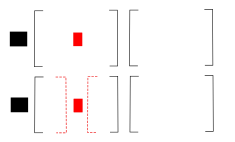
\includegraphics[scale=0.25]{img/attacker_injection_compound.pdf}
	\caption{Example attacker injection when multiple injection points exist in the page. a) a basic injection pattern. b) an attempt to fool the detector.}
	\label{fig:attacker_injection}
\end{figure}

In Figure~\ref{fig:attacker_injection}a, the brackets indicate a template. The content in between is an injection point (the star), where dynamic content is injected into the template. In the case of a vulnerability, the injected content can expand to any arbitrary string. The signature separates the injection from the rest by matching for the start and end points (the \code{endPoints}), represented by the brackets. This HTML originally has two pairs of \code{endPoint} patterns.

In Figure~\ref{fig:attacker_injection}b, the attacker knows these are being used as injection end points and decides to inject a fake ending point and a fake starting point (the dotted brackets), with some additional malicious content in between. If just looking for multiple pairs of end points, the detector cannot tell the difference between the solid and dotted patterns, and will not get rid of the content injected in the star. Therefore, we have to use the first starting point and the last ending point before a starting one (when searching from the bottom-up) and sanitize everything in between. This might get rid of a substantial amount of valid HTML, so we defer to the signature developer's judgement of what behaviour the detector should follow. We expand upon this further in \autoref{case_study}.


\begin{figure}[h]
	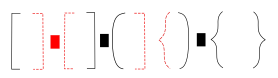
\includegraphics[scale=0.25]{img/attacker_injection_unique.pdf}
	\caption{Example attacker injection when multiple distinct injection points exist in the page.}
	\label{fig:attacker_injection_unique}
\end{figure}


Figure ~\ref{fig:attacker_injection_unique} illustrates a case when there are several injection points in one page, but each of them is distinct. Now, the filter is only looking for one pair of brackets, so the attacker can't fool the extension into leaving part of the injection unsanitized. However, they could, for example, inject an extra ending bracket after the opening parenthesis (or an extra starting brace). The extension will be tricked into sanitizing non-malicious content, the black pluses (+). This behaviour can be detected by noting that we know the order in which the \code{endPoints} should appear, and so if the filter sees a closing \code{endPoint} before the next expected starting \code{endPoint}, or similarly, a starting \code{endPoint} before the next expected closing \code{endPoint}, this attack can be identified. In the diagram, the order of the solid elements characterizes the possible malformations in the end points. As with the previous scenario, we have to sanitize the outermost end points, potentially deleting non-malicious content. The signature developer specifies the sanitization behaviour.

\subsection{Dynamic injections} \label{dynamic_injections}

The top-level documents of web pages fetch additional dynamic content
via \js{fetch} or AJAX APIs. Content fetched in
this way is also vulnerable to \xss, and must be filtered. An example
vulnerability is CVE-2018-7747 (Wordpress Caldera Forms, which allows malicious
content retrieved from the plugin's database to be injected in response to a click.

\sys allows XHR requests to be filtered with \js{xhr}-type
signatures. To reduce the number of signatures that need to be
considered when a browser issues a request, we require that signatures
for XHR be nested inside a signature for a top-level document. If a
page's main content matches an existing top-level signature description,
\sys will then enable all nested XHR listeners.

Signatures for dynamic requests are specified in the \js{listenerData}
key, which includes a listener type and method. The idea is extensible
to scripts and other objects loaded separately from the main document
(e.g., images, stylesheets, etc.).

\lstset{basicstyle=\small}
\begin{lstlisting}[breaklines=true,caption={
      An example dynamic request signature. This patches CVE-2018-7747.
    },label={lst:dynamic_signature}]
...
listenerData: [{
  listenerType: 'xhr', listenerMethod: 'POST',
  sanitizer: 'escape', type: 'string',
  listenerUrl: 'wp-admin/admin-ajax.php',
  typeDet: 'single-unique',
  endPoints: ['<p><strong>', '[AltBody]']
}]
\end{lstlisting}


\section{Implementation}

We have implemented our browser extension in Firefox 67.0.2. Our signatures are currently stored in a local JavaScript file in the extension package.

\subsection{Loading signatures}
As previously mentioned, our detector loads signatures and finds injection points in the document. However, there might be a large number of signatures which don't need to be loaded for a specific website. For example, if several signatures are designed for pages running a WordPress plugin, then the extension need not check any of these for a site which is not running WordPress at all. On the other hand, if a site is running WordPress, we might have to check all signatures meant for WordPress, but not others. Therefore, when loading signatures, we proceed in a manner similar to a decision tree. The detector first probes the page to identify the underlying framework (we call this the 'software' in our signature language). These are usually found by hints in the document HTML. These probes are framework-specific, and as such, need to be encoded in some way so that the detector can run them. There are two approaches for this: the detector completely takes care of this, and needs to be maintained for changes in frameworks and future technologies, or, the signature developer additionally specifies a more specialized version detector as part of a probe file. We chose to go with the first option, as this provides a greater ease of use for signature developers. In our prototype implementation, hard-coding probes detector did not imply a substantial amount of work, however, as more signatures are written and more applications are required to be included, this can become an arduous task. We believe the second option can be desirable and would not be a terrible burden for signature developers: for example, the widely popular network mapping tool Nmap \cite{nMap} uses probes in a similar manner, and these are kept in a modifiable file so that advanced users can have more expressibility. After running these probes, the detector loads signatures for the specific software (e.g. all signatures for WordPress web sites). At this point, we filter out the ones that do not apply to the current page.

\subsection{Version identification}
Finally, we apply version identification. Our objective for versioning is that our signatures don't trigger any false positives on websites running patched software. We found this to be one of the harder aspects of signature loading. In WordPress, for example, many of the plugins do not update their file names with the latest versions, or do not include them at all, and thus, this information is often hard to come by from the client-side perspective. In the case of WordPress, the wp-admin/plugins.php subpath contains information about all currently active plugins on the site. Unfortunately, this information is only available to admins of the site. While this might not be the bulk of users, it is, on the other hand, the bulk of disclosed CVEs, as described in Section 4. Furthermore, we believe that even if we load a signature when the application has already been fixed at the server-side, it will often preserve the page's functionality, as many of the CVEs describe XSS which happens as a result of unsanitized input that was not meant to be JavaScript code regardless. Motivated by this observed behaviour, our mechanism follows a series of increasingly accurate but less applicable version identifiers: first, we apply general-purpose version probes, like the one described for WordPress (these are maintained in a similar way to software probes, hard-coded in the detector logic). If these are not successful, the signature language provides functionality for version identification in the HTML through regex. If the developer considers version information to be unavailable through the HTML, the version in the signature is left blank and the detector applies the signature patch regardless of version, as we can not be sure the page is running patched software.

\subsection{Dynamic injections}
Some of the exploits manifest themselves through dynamically loaded files. For example, CVE-2018-7747 had XSS triggered when the user loaded information stored in the plugin's database after clicking on an element of the page. Since this was not loaded with the original HTML, it came as a response to an Ajax request. Our signature language provides functionality to protect against these kinds of exploits, as shown in the example below:

 \lstset{basicstyle=\small}
\begin{lstlisting}
url: 'wp-admin/admin.php?page=caldera-forms',
...
type: 'listener',
listenerData: {
	listenerType: 'xhr',
	listenerMethod: 'POST',
	sanitizer: 'escape',
	type: 'string',
	url: 'wp-admin/admin-ajax.php',
	typeDet: 'single-unique',
	endPoints: ['<p><strong>', '[AltBody]']
}
\end{lstlisting}

This signature describes an exploit on a WordPress site running the Caldera Forms plugin. The XSS occurs in the specified url. The listenerData attribute defines an extra listener to attach in the background page of the extension. In this case, the page listens for an XHR, specifically done as a POST to the specified subdomain listenerUrl. The rest of the information is similar to a regular signature, as it will execute the filter and sanitize the response if necessary, according to the specified endpoints. The background page knows to only filter such requests originated from the correct web page. The type of resource to listen for is taken as specified by the webRequest API. 

\subsection{Handling multiple injections in one page}
In the previous example, the endPoints were listed as two strings in the incoming network response. However, there are cases where arbitrarily many injection points can be generated by the php code, such as a for loop generating table rows. For these, it is hard to correctly isolate each endPoint pair, as an attacker could easily inject fake endPoints in between the original ones, as shown in the following diagram:

\begin{figure}[h]
	\includegraphics[scale=0.5]{img/attacker_injection.png}
	\label{fig:attacker_injection}
\end{figure}

The content in between black brackets is an injection point. The HTML originally has two pairs of endPoint patterns. The attacker knows these are being used as injection endPoints and decides to inject a fake ending point and a fake starting point, with some additional malicious content in between (shown in red). If the detector were to look for several pairs of endPoints, it would not be able to tell the difference between the red and black patterns, even when using our top-down, bottom-up approach, and would not be able to get rid of the content injected in the red star (\textcolor{red}{*}). Therefore, we have to use first starting point and the last ending point and sanitize everything in between. Depending on the application, this might get rid of a substantial amount of valid HTML, in particular, the web page's functionality might be affected. Due to the difficulty of applying a general solution to this scenario, we defer to the signature developer's judgement, who can specify whether the page should not load at all as part of the signature. We believe this to be preferable to allowing malicious content to be displayed in the page.

A similar case occurs when there are several injection points in one page, but each of them is unique:

\begin{figure}[h]
	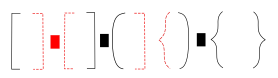
\includegraphics[scale=0.4]{img/attacker_injection_unique.png}
	\label{fig:attacker_injection_unqiue}
\end{figure}

In this case, because the filter is only looking for one pair of brackets, the attacker can't fool the extension into leaving part of the injection unsanitized. However, they could inject an extra ending bracket after the opening parenthesis, or similarly, an extra opening brace before the ending parenthesis. In either case, the extension will be tricked into sanitizing non-malicious content, the black stars (*). We can detect this behaviour by nothing that we know the order in which the endPoints should appear, and so if the filter sees a closing endPoint before the next expected starting endPoint, or similarly, a starting endPoint before the next expected closing endPoint, this attack can be identified. In the diagram, the order is brackets, parenthesis, braces. When it sees a closing bracket after an opening parenthesis, and similarly, when it sees an opening brace before a closing parenthesis, this represents the described attack. As with the previous scenario, we can not easily identify which endPoint is the real one, so sanitization will still potentially get rid of non-malicious content. As before, the signature developer specifies whether the page should be blocked or sanitization goes through as usual when this behaviour is detected.

While our prototype currently does not have a centralized database for signatures, we envision that a trusted entity can maintain this database, such as those that currently maintain CVE databases, and will have to be audited so that it is not filled with false signatures and existing ones are not compromised.
\section{Writing Signatures} \label{signature_writing}

We expect a signature developer to have a solid understanding of the principles behind \ac{XSS}, as well as web applications, HTML, CSS and JavaScript. In this section, we aim to show that minor effort is required from a knowledgeable analyst when writing a signature.


\subsection{Case Study: CVE-2018-10309} \label{case_study}
Going back to our example in Section \ref{motivating_example}, we describe the process by which a signature is written after a vulnerability has been discovered by using one of our studied CVEs.  

\textbf{Identifying the exploit.} An entry in Exploit Database \cite{studyCVE} describes a persistent \ac{XSS} vulnerability in the WordPress plugin Responsive Cookie Consent for versions 1.7/1.6/1.5. This particular entry (as most do) comes with a proof of concept (PoC) for the exploit: 
\begin{enumerate}
	\item Access WordPress control panel.
	\item Navigate to the Responsive Cookie Consent plugin page.
	\item Select one of the input fields. For example, "Cookie Bar Border Bottom Size".
	\item Insert the script you wish to inject.
	\item Save the plugin settings.
	\item Injected script will run in the victim's browser. Depending on which input field you inserted the script, the script may also run everytime you load the Responsive Cookie Consent plugin page.
	
\end{enumerate}

\textbf{Establishing the separation between dynamic and static content.} We insert the string \js{"$>$script$>$alert('XSS')$<$/script$>$} in the rcc\_settings[border-size] input field, as detailed by the PoC. This results in an alert box popping up in the page, which has the  following HTML:

\begin{lstlisting}
<input id="rcc_settings[border-size]" 
name="rcc-settings[border-size]" 
type="text" value=<@\textcolor{red}{""><script>alert('XSS')</script>}@>
<label class="description"
for="rcc_settings[border-size]">
\end{lstlisting}

In general, the CVE writer is able to find the vulnerable HTML from the server-side code without having to reproduce the exploit. Since we did not write the CVE, we had to do this extra step.

In this case, it is clear that the \textbf{input} element is the injection starting point, and we use the \textbf{label} element as the end point, since it is the element immediately after the \textbf{input}. We must emphasize that the identification of correct endpoints is extremely important. In particular, when multiple injection points exist in the same page, the signature developer must be cautious with the chosen elements, and ensure that these do not overlap with other innocuous ones. In some cases, the developer might find it best to completely stop the page from loading if they think the sanitization would affect the user experience too greatly. While one of our main goals is to maintain the page’s usability, there are cases where a large portion of the document would be affected by the sanitization, and we believe compromising usability for security is preferable in this case. Furthermore, the developer has to identify whether the exploit comes in from an external source (such as an Ajax request) or is embedded in the document’s mainframe HTML. 

\textbf{Collecting other required page information and writing the signature.} The next step is to gather the remaining information to determine whether the signature applies to the page loaded. The full signature for this example was previously shown in Listing \ref{lst:xsnare_signature}. The \textbf{URL} is acquired by noting that this exploit occurs on the plugin's settings page. The \textbf{software} running is WordPress in this case. The settings page's HTML includes a link to a stylesheet with href "http://localhost:8080/wp-content/plugins/responsive-cookie-consent/includes/css/options-page.css?ver=5.2.2", in particular, "wp-content/plugins/plugin-name" is the standard way of identifying that a WordPress page is running a certain plugin. In this case, "responsive-cookie-consent", set as \textbf{softwareDetails}. We apply the signature for all versions less than or equal to 1.7. Since, the exploit only occurs in this specific spot in the HTML, the \textbf{typeDet} is listed as 'single'. 
Since the vulnerable parameter is for border-size, the \textbf{sanitizer} applied is 'regex', further restricting the pattern to only numbers in \textbf{config}. Finally, we list the \textbf{endPoints} as taken from the HTML.

\textbf{Testing the signature}. Finally, we load up our extension and reload the web page. In this example, we expect to not have an alert box pop up, and we manually look at the HTML to verify correct sanitization. Note that there's nothing else in between the \textbf{input} and \textbf{label} elements now:

\begin{lstlisting}
<input value="" type="text" 
name="rcc_settings[border-size]" 
id="rcc_settings[border-size]">
<label class="description"
for="rcc_settings[border-size]">
\end{lstlisting}

In practice, there might be small discrepancies between server-side and client-side representations of the HTML string, leading to bugs in the signature if the developer used the parsed HTML as a reference. If the exploit is not properly sanitized, the developer is able to use the debugging tools provided by the browser to check the incoming network response information seen by the extension's background page and make sure it matches the signature values.

\iffalse
\subsection{Signature writing process}
We describe the process by which a signature is written after a vulnerability has been discovered:
\begin{enumerate}
	\item{
The signature developer crafts a proof of concept exploit for the given CVE. This step is not necessary but it will often help the developer correctly identify the affected areas of the DOM. For our own signatures, we heavily relied on this part because we often did not have the same information as the CVE writer.
Conversely, a knowledgeable analyst will often be able to identify the vulnerable points in the application from the server-side code.}
\item
Using information about where in the HTML the exploit will manifest itself, the developer identifies the start and end points of an injection, and creates regexes to match these. This step is particularly important because this is where the signature might end up covering a bigger part of the DOM than is required, potentially disabling desired functionality, to the detriment of the site user's experience. In particular, when multiple injection points occur in the same page, the developer might find it best to completely stop the page from loading if they think the sanitization would affect the user experience too greatly. While one of our main goals is to maintain the page's usability, there are cases where a large portion of the document would be affected by the sanitization, and we believe compromising usability for security is preferable in this case.

Furthermore, it is at this point where the developer identifies whether the exploit comes in from an external source (such as a response to an Ajax request or an external script) or is embedded in the document's mainframe HTML. This will result in a different signature layout. 
\item
Signatures are loaded for specific pages, and the developer has to specify this information, either via an URL or a regex in the HTML. For example, for a WordPress plugin, the exploit might happen in localhost/plugin-name.php. However, for another exploit, the exploit might occur in a page where the plugin is loaded, which contains the string "wp-content/plugins/plugin-name" in the HTML. Additionally, if the webpage is running pre-defined software, such as WordPress, this has to be specified in the signature as well. Much of this information is already known beforehand, and so this step can be done in conjunction with Step 2.
\item
After the signature has been written, the developer should make sure it was correctly specified. This is most easily done via testing a PoC exploit and verifying the injection has been properly sanitized. For false positives, the developer should make sure that the specified endPoints are uniquely occurring in the HTML (or if not unique, their correct positions have been stated). The browser extension can be used for the purposes of debugging. Some of our most common mistakes when writing signatures were incorrect regexes for the endpoints, and not correctly identifying that the injection occurred as part of an additional network request. These two can be easily fixed by looking through the incoming HTML in the background page's filter. 
\end{enumerate}

\subsection{Case Study: CVE-2018-10309}
Going back to our example in Section 2.4, we describe the full process of writing a signature for one of the CVEs we studied. An entry in Exploit Database \cite{studyCVE} describes a persistent \ac{XSS} vulnerability in the WordPress plugin Responsive Cookie Consent for versions 1.7/1.6/1.5. This particular entry (as most do) comes with a proof of concept for the exploit: 
\begin{enumerate}
\item Access WordPress control panel.
\item Navigate to the Responsive Cookie Consent plugin page.
\item Select one of the input fields. For example, "Cookie Bar Border Bottom Size".
\item Insert the script you wish to inject.
\item Save the plugin settings.
\item Injected script will run in the victim's browser. Depending on which input field you inserted the script, the script may also run everytime you load the Responsive Cookie Consent plugin page.
	
\end{enumerate}

 As described in Section 4.1, in order to test this vulnerability, we find a link to the affected plugin code, and launch a container with a clean installation of WordPress 5.2 with the plugin downloaded. After this, we activate the plugin and proceed to reproduce the proof of concept as described in the Exploit Database entry, inserting the string '">script>alert('XSS')</script>' in the rcc\_settings[border-size] input field, resulting in the following HTML displayed on the page, as well as an alert box popping up in the page:

\begin{lstlisting}
<input id="rcc_settings[border-size]" 
name="rcc-settings[border-size]" 
type="text" value=<@\textcolor{red}{""><script>alert('XSS')</script>}@>
<label class="description"
for="rcc_settings[border-size]">
\end{lstlisting}

In this case, it is clear that the \textbf{input} element is the injection starting point, and we use the \textbf{label} element as the end point, since it is the immediate element after the \textbf{input}. With this information, we are now ready to start writing the corresponding signature, as shown in Listing \ref{lst:xsnare_signature}.

\iffalse
 \lstset{basicstyle=\small}
\begin{lstlisting}
url: 'wp-admin/options-general.php?page=rcc-settings',
software: 'WordPress',
softwareDetails: 'responsive-cookie-consent',
version: '1.7',
type: 'string',
typeDet: 'single-unique',
endPoints: 
['<input id="rcc_settings[border-size]" 
name="rcc_settings[border-size]" type="text"',
'<label class="description" 
for="rcc_settings[border-size]">']
\end{lstlisting}
\fi

The URL is acquired by noting that this exploit occurs on the plugin's settings page, which is in a specific subdomain of the web site. Of course, the software running is WordPress in this case. The settings page's HTML includes a link to a stylesheet with href "http://localhost:8080/wp-content/plugins/responsive-cookie-consent/includes/css/options-page.css?ver=5.2.2", in particular, "wp-content/plugins/plugin-name" is the standard way of identifying that a WordPress page is running a certain plugin. In this case, "responsive-cookie-consent". While the entry only lists versions 1.7, 1.6, and 1.5 as vulnerable, we apply the signature for all versions less than or equal to 1.7.
Since, the exploit only occurs in this specific spot in the HTML, the typeDet is listed as "single-unique". Finally, we list the endPoints as taken from the HTML.

Finally, we load up our extension and reload the web page. In this example, we expect to not have an alert box pop up, and we manually look at the HTML to verify correct sanitization. Note that there's nothing else in between the input and label elements now:

\begin{lstlisting}
<input value="" type="text" 
name="rcc_settings[border-size]" 
id="rcc_settings[border-size]">
<label class="description"
for="rcc_settings[border-size]">
\end{lstlisting}

\fi

\section{Approach evaluation} \label{viability}

To verify the applicability of our detector and signature language, we tested the system by looking at several recent CVEs related to \ac{XSS}. We have three objectives: to verify that our signature language provides the necessary functionality to express an exploit and its patch, to test our detector against existing exploits, and to show that composing signatures takes a reasonable amount of time.

% does not incur a high time overhead when writing a signature.

\subsection{Methodology} \label{methodology}

We study recent CVEs related to WordPress
plugins. We focus on WordPress for two reasons:
%% While this may seem restrictive, there are several reasons
%% why we targeted WordPress plugins:
\begin{enumerate}
	\item WordPress powers 34.7\% of all websites according to a recent survey  \cite{w3stats} \cite{DBLP:journals/corr/abs-1801-01203}. The same study states that 30.3\% of the Alexa top 1000 sites use WordPress. Thus, we can be confident that our study results will hold true for the average user.
	\item WordPress plugins are popular among developers (there are currently more than 55,000 plugins \cite{wpplugins}). Due to its user popularity, WordPress is also heavily analyzed by security experts. A search for WordPress CVEs on the Mitre CVE database \cite{cvemitre} gives 2310 results. Plugins, specifically, are an important part of this issue, 52\% of the vulnerabilities reported by WPScan are caused by WordPress plugins \cite{wpscan}.
	%% \item WordPress plugin code is accessible, so we can easily analyze both the client-side HTML, as well as the server-side code that generated it, which is helpful when writing signatures.
	%% \item Using one framework, we can install many different plugins for the version we want, reproduce attacks, and investigate the conditions under which they happen, without having to install additional software.
\end{enumerate}

We used a CVE database, CVE Details~\cite{cvedetails} to
find the 100 most recent WordPress \ac{XSS} CVEs, as of
October 2018. %% We used a CVE database, CVE Details
%% \cite{cvedetails}, as opposed to other databases that include
%% vulnerabilities or exploits, mainly because of reliability. We have
%% been able to find hundreds of verified attacks on WordPress and its
%% plugins using a CVE database, which also usually contain information
%% on how to reproduce them. This provides the perfect platform to
%% analyze \ac{XSS} attacks and decide whether they can be countered by
%% our approach.
%
For each CVE, we set up a Docker container with a clean installation
of WordPress 5.2 and installed the vulnerable plugin's version. 
For CVEs that depended on a particular WordPress version, we
installed the appropriate version. Of the CVEs we looked at, only
one occurred in WordPress core. We believe it would be harder
to precisely sanitize injection points in WordPress core, as many of
the plugins have particular settings pages where the exploits occur,
and the HTML is more identifiable. WordPress core, on the other hand,
can be heavily altered by the use of themes and the user's own
changes. However, as evidenced by our investigation, the vast majority
of exploits occur in plugins.
 
Next, we reproduced the exploit in the CVE and we analyzed the
vulnerable page and wrote a signature to patch the exploit.

%%%%%%%%%%%%%%%%%%%%%%%%
\subsection{Results}
%%%%%%%%%%%%%%%%%%%%%%%%

\begin{table}[h!]
	\begin{center}
		\begin{tabular}{c c} 
			\hline
			\textbf{Plugin} & \textbf{Installations}\\ [1ex] 
			\hline
			WooCommerce  & 5+ million  \\  
			Duplicator & 1+ million \\  
			Loginizer & 900,000+ \\  
			WP Statistics & 500,000+ \\  
			Caldera Forms & 200,000+ \\   
			\hline
		\end{tabular}
		\caption{Most popular studied WordPress plugins}
		\label{table:1}
	\end{center}
\end{table}

Of the initial 100 CVEs, we were able to analyze 76 across 44 affected
pages. We dropped 24 CVEs due to reproducibility issues: some of the
descriptions did not include a PoC, making it difficult for us to
reproduce; or, the plugin code was no longer available. In some cases,
it had been removed from the WordPress repository due to "security
issues", which emphasizes the importance of being able to defend
against these attacks. %% This is not to say, however, that our detector
%% would not work for such a CVE, as the author would have a better idea
%% of how the exploit manifests itself, and would be in a better position
%% to write a signature.

The resulting plugins we studied averaged 489,927
installations: \autoref{table:1} shows the number of installations for
the 5 most popular plugins we studied. For the vulnerabilities, 27
(35.5\%) could be exploited by an unauthenticated user; 56 (73.7\%)
targeted a high-privilege user as the victim, 7 (9.2\%) had a
low-privilege user as the victim, the rest affected users of all
types.

Many of the studied CVEs included attacks for which there are known
and widely deployed defenses. For example, many were cases of
Reflected \ac{XSS}, where the URL revealed the existence of an attack,
e.g.,: \url{http://<target>\&page-uri=<script>alert("XSS")</script>}
While Chrome's built-in \ac{XSS} auditor blocked this request, Firefox
did not, and so we still wrote signatures for such attacks\footnote{In
practice, we found several cases where even XSS auditor did not block
a reflected XSS.}.

We wrote 59 WordPress signatures in total, which got rid of the PoC
exploit when sanitized with one of our three methods. Note that while
a PoC is often the most simple form of an attack, our sanitization
methods, and in particular DOMPurify, can get rid of complex
injections as well. We were able to include several CVEs in some PoCs
because they occurred in the same page and affected the same
plugin. Overall, these signatures represent 71 (93.4\%) signed
CVEs. The 5 we were not able to sign were due to lack of identifiers
in the HTML, which would result in potentially large chunks of the
document being replaced\footnote{In these cases, the signature developer
can weigh the trade-offs and decide whether the added cost is worth
it.}

After manual testing, the majority of the 71 signatures maintained the
same layout and core functionality of the webpage. However, 12
signatures caused some elements to be rearranged, modifying the page's
visual aspect. One caused a small part of the page to become unusable,
due to the sanitization method (a table showing user information
was now rendered as blank). Most of the responsibility of maintaining
functionality is left to the signature developer. We found that being precise
is key to retaining functionality. Furthermore, even if the layout of the page is
affected, we believe that applying the signature is preferable
to allowing an exploit. And, unlike the complete blocking approach commonly used by malware
detection software, our approach allows the user to access the page.

While our goal is to retain as much information of the page as
possible after sanitization, we believe that even if a part of the
page becomes unusable, this does not impact the user's experience as
much, since many of the exploits occur in small sections of the
HTML. A usability study is out of scope for this paper and we leave it
to future work.

%%  (see , but we provide some insight into false positives and false
%% negatives in 
%, which is related to this issue.

\subsection{Generalizability beyond WordPress}
\label{generalizability}

To test the generalizability of our approach to other frameworks, we
analyzed 5 additional CVEs, 2 related to Joomla!, 2 for LimeSurvey,
and 1 for Bolt CMS.  We chose Joomla! because it is another
popular \ac{CMS}. Unfortunately, we only found 2 CVEs
that we were able to reproduce, as the software for its extensions is
often not available. For fairness, we looked for the most recent CVEs
we could reproduce listed in the Exploit Database~\cite{exploitdb}, since
these have recorded \acp{PoC}. We carried out the same
procedure as with the WordPress CVEs, and were able to patch all of
the 5 exploits. This brought our CVE coverage rate up to 93.8\%.

\subsection{Signature writing times} \label{signature_times}

\autoref{fig:signature_times} plots a histogram of the times it took
one of the authors to compose each of the signatures. Each time
measurement includes the time it took to check the HTML injection
points, write the signature and to debug it. We do not include the
time taken to discover and carry out an exploit, as this is part of
the CVE writing process. The median time is 3.89 minutes, and the
standard deviation is 4.18 minutes. 72\% of signatures were written in
under 5 minutes. We believe this to be a reasonable amount of time
considering the security granted by our extension.

The signature which took the longest time to write (25 minutes)
corresponds to an exploit with 12 HTML injection points. Additionally,
testing this signature proved difficult, as some of
the injections were a result of a script inserting elements in the DOM
after the page had loaded. This caused the initial HTML to look
innocuous, but with exploits still occurring after sanitization. As
this script was part of the initial request, we eventually got to the
root of the problem. We believe a more experienced exploit analyst
might be able to detect this kind of behaviour more
easily. %% Furthermore, having so many injection points in the HTML is
%% cause for great complexity, and the writer can decide to block the
%% page entirely, which would bring down the time taken.

The signature which took the second longest time to write (18 minutes)
corresponds to an exploit with 7 injection points; each of
these belongs to a part of the HTML with generic element
identifiers. Our language provides a means to overcome this, by allowing
the developer to specify the element's "position": for example, if there are
three $<$h3 class="title"$>$ elements, in the HTML, and only one of them
is an injection starting point, the writer can specify that the third
one needs to be sanitized. The same can be done for the ending points. As
there were 7 of such points, debugging took longer than for
other signatures.
%% Again, this is a complex case, and can be
%% more prone to user error than other signatures, the writer might
%% instead decide to block the page entirely.

%% Our dataset contained signatures which cover several CVEs, as
%% sometimes a single page is associated with multiple CVEs. We had 6
%% such pages. which had a median write time of 6.54 minutes. This means
%% that the time per CVE is lower than the overall median of
%% 3.89.
Another source of longer timings are complicated 
listener type signatures, like the ones for exploits caused by an
XHR. We had 4 such signatures and composed these with a median time of 9.86 minutes.
%% these had a median write time of 9.86.
As only a small number of these were present, we expect the time
taken to compose a typical signature to be lower than the overall median in this experiment.

\begin{figure}[h]
	\begin{center}
	\includegraphics[width=\linewidth]{results/signature_times_small.pdf}
	\caption{Histogram of time taken to write signatures.}
	\label{fig:signature_times}
	\end{center}
\end{figure}



\section{Performance Evaluation}
The extension's performance goals are to provide our security guarantees without being a detriment to the end user's browsing experience. All of our timestamps were recorded using the Performance Web API. While our extension's functionality only applies at the network level, there is potential slowdown at the DOM processing level. Figure ~\ref{fig:navigationtiming} presents shows the different timestamps provided by the Navigation Timing API, as well as a high-level description of the browser processing model. Since our filter listens on the onBeforeRequest event, none of the previous steps before Request are affected. In this section, we refer to the difference in time between responseEnd and requestStart as the "network filter time".

\begin{figure}[h]
 \includegraphics[scale=0.32]{img/timestamp-diagram}
 \caption{The Navigation Timing API's timestamps}
 \label{fig:navigationtiming}
 \end{figure}

\subsection{Top websites load times}
We first report our extension's impact on top website load times, representing the expected behaviour of an user's average web browsing experience. For these tests, we first took the top 500 websites as reported by Moz.com \cite{top500}. For each website, we loaded it 20 times (with a 25 second timeout) and recorded the following values: requestStart, responseStart, responseEnd, domContentLoadedEventEnd, domComplete, duration, and decodedBodySize. From the initial 500, we only report values for 441 of them. The other 59 had consistent issues with timeouts, insecure certificates, and network errors. For our setup, we used a headless version of Firefox, and Selenium WebDriver for NodeJS, with GeckoDriver. We ran four test suites:
\begin{itemize}
	\item No extension cold cache: Firefox is loaded without the extension installed and the web driver is re-instantiated for every page load.
	\item Extension cold cache: Firefox is loaded with the extension installed and the web driver is re-instantiated for every page load.
	\item No extension warm cache: Firefox is loaded without the extension installed and the same web driver is used for the page's 20 loads.
	\item Extension warm cache: Firefox is loaded with the extension installed and the same web driver is used for the page's 20 loads.
\end{itemize}

The recorded timestamps do not hold much value by themselves, only when analysed with regards to each other. Thus, for each set of tests, we reduced the recorded values to three comparisons: responseStart (responseStart - requestStart), responseEnd (responseEnd - requestStart), and domResponse (domComplete - responseStart). The first two analyze the time spent by the network filter, while the third determines the time spent until the whole document has loaded. We calculate the medians of each website for each of the previous three values and the decodedByteSize.

Finally, we compare the load times with and without the extension running by calculating the relative slowdown with the extension installed. Figure ~\ref{fig:overall_slowdown} shows the computed results. The graph shows that the slowdown is not too great when the extension is running. Note that these values are recorded as percentages, and while some are as high as 200\%, the absolute values are in the order of seconds, and in many cases tens or hundreds of milliseconds, especially for the network component. The slowdown increases when we take caching into account. We expect this to be the case because the network filter probably causes the browser to use less caching, especially for the DOM component, as it might have to process it from scratch every time.

Figure ~\ref{fig:histogram_slowdown} shows a closer look at the distribution for the network filter slowdown on the top sites. We see that for this component, most of the slowdown is centred around [-10\%,10\%].

Figure ~\ref{fig:network_filter_decoded_size} shows the network filter time as a function of the page's decoded byte size. Since the probes perform regex matching, the upwards trend line is expected. However, we see that almost all the sites up to 1.2 MB take under 500 ms.

Additionally, for each website we recorded the number of loaded signatures (i.e. signatures whose endpoints were found in the HTML). None of the websites loaded any signatures, even though some of the probes tested positive for WordPress sites (recall our implementation currently only has probes for WordPress). Thus, we can infer with confidence that the rate of false positives for loaded signatures during an average user's web browsing is extremely low. While we can not be sure that any of the sites is free of vulnerabilities described in our current signatures, this is very unlikely, as many of these websites are not running WordPress to begin with, and being some of the most popular, they would likely be updated relatively quickly if any vulnerability is found; thus, the rate of false negatives is likely extremely low as well. It is reasonable to assume that the rate of false positives for loaded signatures would go up for a WordPress site. Since most of the tested sites are not running WordPress, this might have skewed the probability down. TODO: can we calculate a conclusive value for false positives of loaded signatures out of the number of websites running wordpress on the top 1000?

\begin{figure}[h]
	\includegraphics[scale=0.5]{results/extension_slowdown_overall}
	\caption{Cumulative distribution of relative percentage slowdown with extension installed for top sites}
	\label{fig:overall_slowdown}
\end{figure}

\begin{figure}[h]
	\includegraphics[scale=0.5]{results/density_histogram_filter_slowdown}
	\caption{Density histogram of network filter slowdown for top sites}
	\label{fig:histogram_slowdown}
\end{figure}

\begin{figure}[h]
	\includegraphics[scale=0.5]{results/byte_size_vs_filter_time}
	\caption{Scatter plot of network filter time as a function of decoded byte size for top sites}
	\label{fig:network_filter_decoded_size}
\end{figure}


\section{Limitations and Future Work}
\textbf{Generalizability.} Our study has only covered WordPress websites. While many websites, in particular ones that use any kind of CMS might share similar structures to the ones we studied, it is clear that the open source nature and availability of WordPress code and its plugins might have made our assumption of full knowledge of the HTML too strong. We acknowledge that this assumption will not always hold true, however, many websites will still be able to benefit from our approach.

\textbf{Scope of study.} Our current CVE study has only covered 100 CVEs, 23 of which had to be discarded in our result analysis. We intend to cover more in the future to have a better representation of WordPress websites and plugins and the web as a whole. 

\textbf{Current implementation.} There are several aspects of injections that we have not been able to test as a result of the CVEs not exploiting these, like attacks through images. Our prototype implementation lacks several performance enhancements which would greatly benefit the overhead caused by the extension, like parallelizing signature loading and sanitization, as well as using more efficient data structures to store signatures. 

\textbf{False positives and false negatives.} Due to the nature of our approach, it is nigh impossible to completely get rid of false positives. While we concluded that the rate of false positives is ver low for loaded signatures, these can still occur when a signature is correctly loaded, since the sanitization might get rid of elements that were intended to be there. We have previously discussed the ability to reproduce the developer's intention with regards to when scripts should be able to run, however, this won't always be possible, as there will be cases where there are injection points where non-malicious JavaScript is allowed, and thus, our system will have false positives. Furthermore, since we rely on handwritten signatures to defend against attacks, it is possible that not every single injection point of every website will be covered, and so we will also have false negatives. In the future, we intend to study the rate of false positives and negatives in our approach and compare it to previous work. Faulty sanitization could be reduced by implementing our sanitization methods as a lexer instead of the declarative version we currently have: The signature developer would ideally provide the allowed behaviour in a given injection point, and the detector would check the injection content against the signature-specified behaviour, providing a proof of whether the content could have been generated by following the rules, and if not, eliminating any content that could not be have been generated from them.

\textbf{Usability.} A main aspect of our work is its increased potential for usability and adoption from both an user's perspective that installs the extension to defend themselves against XSS, and a signature developer that has to write the database descriptions according to a known CVE. Future work could focus on usability studies related to both of these components.

\textbf{Protection against CSRF.} While our work has only focused on XSS, we believe we can easily adapt our network filter to defend against CSRF exploits as well. Using a similar signature language as the one for XSS, a signature developer could specify pages with potential vulnerabilities and enforce network requests that can not exploit such vulnerabilities. In some scenarios, it might be useful to track DOM events, e.g. user clicks to protect against clickjacking attacks. This kind of information is not available to the network; however, the extension could install a script on the page to monitor these actions. 

\textbf{Dealing with an increasing amount of signatures.} Our naive approach at signature filtering (once a probe for a framework has passed) has been effective with our current amount of signatures. However, as the number of signatures increases, and more types of sites are covered, the performance impact may increase drastically. As of September 2019, CVE Details had 14894 XSS vulnerabilities in its database \cite{vulnbytype}. This would mean that our current signatures only cover 0.5\% of all existing XSS vulnerabilities. In reality, the figure would not be as small, since many of these vulnerabilities are old and the software to which they applied has already been updated, making the probability of encountering an exploit very low. Regardless, more efficient approaches at searching and filtering, as well as for the data structures used in the signature database could be applied to maintain a low performance overhead. (TODO: someone might know or have referenced to what firewalls do?)

\section{Related Work}
We classify existing work into several categories: client-side, server-side, browser built-in, and hybrid approaches.

\textbf{Server-side techniques.}
In addition to existing parameter sanitization techniques,
taint-tracking has been proposed as a means to consolidate
sanitization of vulnerable parameters, and identify vulnerabilities automatically. ~\cite{10.1145/1368088.1368112, Xu:2006:TPE:1267336.1267345,DBLP:conf/sec/Nguyen-TuongGGSE05,Pietraszek:2005:DAI:2146257.2146267,Bisht:2008:XPD:1428322.1428325, 5070521}. These techniques are complementary to ours, and provide an additional line
of defence against \ac{XSS}.
% However, many of them rely on the
%client-side rendering to maintain the server-side properties, which
%will not always be the case.

There has also been work on other server-side analysis approaches
to find bugs security vulnerabilities in web applications. \cite{10.1145/1390630.1390661, 5416728, 10.1145/2393596.2393608}.
However, these do not target XSS specifically.

\textbf{Client-side techniques.}
DOMPurify~\cite{10.1007/978-3-319-66399-9_7} presents a robust
\ac{XSS} client-side filter. The authors
argue that the DOM is the ideal place for sanitization to occur. While
we agree with this view, this work relies on application developers
to adopt the filter and modify their code to use it. We have partly automated this step by including it as our default sanitization function.

Jim et al.~\cite{Jim:2007:DSI:1242572.1242654} present a method to
defend against injection attacks through Browser-Enforced Embedded
Policies. This approach is similar to ours, as the policies specify
prohibited script execution points. Similarly, Hallaraker and Vigna~\cite{Hallaraker:2005:DMJ:1078029.1078861} use a
policy language to detect malicious code on the client-side. Like \sys, they make use of signatures to protect against known types of
exploits. However, unlike our approach, their signatures are not
application-specific, and there is no model for signature
maintenance.

Snyder et al.~\cite{Snyder:2017:MWD:3133956.3133966} report a study in which
they disable several JavaScript APIs and test the number of websites
that are do not work without the full functionality of the APIs. This approach increases security due to vulnerabilities present in several
JavaScript APIs, however, we believe disabling API functionality
should only be used as a last resort.

Additionally, client-side taint tracking, through the use of static and dynamic analysis,
 has also been applied as a means to detect XSS, either
at the browser level or at the extension level \cite{8094406, 10.1007/978-3-642-04444-1_33}.

\textbf{Browser built-in defences.}  Browsers are equipped
with several built-in defences. We previously described XSS
Auditor in \autoref{introduction}. Another important one is the 
 \ac{CSP}~\cite{CSP}. It has been widely adopted and
in many cases provides developers with a reliable way to protect
against \ac{XSS} and \ac{CSRF} attacks. However, \ac{CSP} requires the developer to identify which scripts
might be malicious. Previous work has also highlighted the need for further built-in defences \cite{6825636}.

\textbf{Client and server hybrids.}
XSS-Dec~\cite{Sundareswaran:2012:XHS:2352970.2352994} uses a proxy which keeps track of an encrypted version of the server's source files, and applies this information to derive exploits in a page visited by the user. This approach is similar to ours, since we assume previous
knowledge of the clean HTML document. Furthermore, they use anomaly-based and signature-based detection to prevent attacks. Our system offloads all this functionality to the client-side, without the need for any server-side information.


\section{Conclusions}
We have presented XSnare, a fully client-side protection mechanism against XSS. This approach has many benefits over currently existing systems, as well as being complementary to many of them. Our firewall architecture makes it so that users can protect themselves in the face of an ever-increasing number of potential attacks and attack vectors, with very little additional user effort required. The CVE study we conducted shows that a majority of websites can benefit from our defence strategy and, thus, we conclude that this is a viable system. Our prototype implementation meets the required performance goals to not be detrimental to an user's web browsing experience. We continue working on the system to become more robust both in terms of being able to defend against a myriad of attacks, as well as providing ease of development for signatures. 

%\appendix
\section{Signature Language Specification} \label{appendix:language_specification}
We provide a description of our signature language, in particular in the context of WordPress:
\begin{itemize}
	\item
	url: If the exploit occurs in a specific URL or subdomain, this is defined as a string, e.g.
	\url{/wp-admin/options-general.php?page=relevanssi\%2Frelevanssi.php}, otherwise null.
	\item
	software: The software framework the page is running if any, e.g. WordPress. A hand-crafted page
	might not have any identifiable software.
	\item
	softwareDetails: If running any software, this provides further information about when to load a signature. For WordPress, these are plugin names as depicted in the HTML of a page running such plugin.
	\item
	version: The version number of the software/plugin/page. This is used for versioning as described earlier.
	\item 
	type: A string describing the signature type. A value of "string" describes a basic signature. A value of 'listener' describes a signature which requires an additional listener in the background page for network requests.
	\item 
	sanitizer: A string with one of the following values: "DOMPurify", "escape", and "regex". This item is optional, the default is DOMPurify.
	\item
	config: The config parameters to go along with the chosen sanitizer, if necessary. For "DOMPurify", the accepted values are as defined by the DOMPurify API (i.e DOMPurify.sanitize(dirty, config). For "escape", an additional escaping pattern can be provided. For "regex", this should be the pattern to match with the injection point content.
	\item
	typeDet: A string with the following pattern: 'occurrence-uniqueness'. As described in Section 2.4, this specifies whether there are several injection points in the HTML.
	\item
	endPoints: An array of startpoint and endpoint tuples.
	\item 
	endPointsPositions: An array of integer tuples. These are optional but useful when the one of the endPoints HTML are used throughout the whole page and appear a fixed number of times. For example: if an injection ending point happens on an element <h3 class='my-header'>, this element might have 10 appearances throughout the page. However, only the 4th is an injection ending point. The signature would specify the second element of the tuple to be 7, as it would be the 7th such item in a regex match array (using 1-based indexing), counting from the bottom up. For ending points, we have to count from the bottom up because the attacker can inject arbitrarily many of these elements before it, and vice versa for starting points.
\end{itemize}

Additionally, if the value of type is 'listener', the signature will have an additional field called listenerData. Similarly to a regular signature, this consists of the following pieces of information:
\begin{itemize}
	\item 
	listenerType: The type of network listener as defined by the WebRequest API (e.g. 'script, 'XHR', etc.)
	\item
	listenerMethod: The request's HTTP method, for example "GET" or "POST".
	\item
	url: the URL of the request target.
\end{itemize}

\bibliographystyle{ACM-Reference-Format}
\bibliography{references}

\end{document}
